\documentclass[]{article}
\usepackage{lmodern}
\usepackage{amssymb,amsmath}
\usepackage{ifxetex,ifluatex}
\usepackage{fixltx2e} % provides \textsubscript
\ifnum 0\ifxetex 1\fi\ifluatex 1\fi=0 % if pdftex
  \usepackage[T1]{fontenc}
  \usepackage[utf8]{inputenc}
\else % if luatex or xelatex
  \ifxetex
    \usepackage{mathspec}
  \else
    \usepackage{fontspec}
  \fi
  \defaultfontfeatures{Ligatures=TeX,Scale=MatchLowercase}
\fi
% use upquote if available, for straight quotes in verbatim environments
\IfFileExists{upquote.sty}{\usepackage{upquote}}{}
% use microtype if available
\IfFileExists{microtype.sty}{%
\usepackage{microtype}
\UseMicrotypeSet[protrusion]{basicmath} % disable protrusion for tt fonts
}{}
\usepackage[margin=1in]{geometry}
\usepackage{hyperref}
\hypersetup{unicode=true,
            pdftitle={Homework 5},
            pdfauthor={Christophe Hunt},
            pdfborder={0 0 0},
            breaklinks=true}
\urlstyle{same}  % don't use monospace font for urls
\usepackage{color}
\usepackage{fancyvrb}
\newcommand{\VerbBar}{|}
\newcommand{\VERB}{\Verb[commandchars=\\\{\}]}
\DefineVerbatimEnvironment{Highlighting}{Verbatim}{commandchars=\\\{\}}
% Add ',fontsize=\small' for more characters per line
\usepackage{framed}
\definecolor{shadecolor}{RGB}{248,248,248}
\newenvironment{Shaded}{\begin{snugshade}}{\end{snugshade}}
\newcommand{\KeywordTok}[1]{\textcolor[rgb]{0.13,0.29,0.53}{\textbf{{#1}}}}
\newcommand{\DataTypeTok}[1]{\textcolor[rgb]{0.13,0.29,0.53}{{#1}}}
\newcommand{\DecValTok}[1]{\textcolor[rgb]{0.00,0.00,0.81}{{#1}}}
\newcommand{\BaseNTok}[1]{\textcolor[rgb]{0.00,0.00,0.81}{{#1}}}
\newcommand{\FloatTok}[1]{\textcolor[rgb]{0.00,0.00,0.81}{{#1}}}
\newcommand{\ConstantTok}[1]{\textcolor[rgb]{0.00,0.00,0.00}{{#1}}}
\newcommand{\CharTok}[1]{\textcolor[rgb]{0.31,0.60,0.02}{{#1}}}
\newcommand{\SpecialCharTok}[1]{\textcolor[rgb]{0.00,0.00,0.00}{{#1}}}
\newcommand{\StringTok}[1]{\textcolor[rgb]{0.31,0.60,0.02}{{#1}}}
\newcommand{\VerbatimStringTok}[1]{\textcolor[rgb]{0.31,0.60,0.02}{{#1}}}
\newcommand{\SpecialStringTok}[1]{\textcolor[rgb]{0.31,0.60,0.02}{{#1}}}
\newcommand{\ImportTok}[1]{{#1}}
\newcommand{\CommentTok}[1]{\textcolor[rgb]{0.56,0.35,0.01}{\textit{{#1}}}}
\newcommand{\DocumentationTok}[1]{\textcolor[rgb]{0.56,0.35,0.01}{\textbf{\textit{{#1}}}}}
\newcommand{\AnnotationTok}[1]{\textcolor[rgb]{0.56,0.35,0.01}{\textbf{\textit{{#1}}}}}
\newcommand{\CommentVarTok}[1]{\textcolor[rgb]{0.56,0.35,0.01}{\textbf{\textit{{#1}}}}}
\newcommand{\OtherTok}[1]{\textcolor[rgb]{0.56,0.35,0.01}{{#1}}}
\newcommand{\FunctionTok}[1]{\textcolor[rgb]{0.00,0.00,0.00}{{#1}}}
\newcommand{\VariableTok}[1]{\textcolor[rgb]{0.00,0.00,0.00}{{#1}}}
\newcommand{\ControlFlowTok}[1]{\textcolor[rgb]{0.13,0.29,0.53}{\textbf{{#1}}}}
\newcommand{\OperatorTok}[1]{\textcolor[rgb]{0.81,0.36,0.00}{\textbf{{#1}}}}
\newcommand{\BuiltInTok}[1]{{#1}}
\newcommand{\ExtensionTok}[1]{{#1}}
\newcommand{\PreprocessorTok}[1]{\textcolor[rgb]{0.56,0.35,0.01}{\textit{{#1}}}}
\newcommand{\AttributeTok}[1]{\textcolor[rgb]{0.77,0.63,0.00}{{#1}}}
\newcommand{\RegionMarkerTok}[1]{{#1}}
\newcommand{\InformationTok}[1]{\textcolor[rgb]{0.56,0.35,0.01}{\textbf{\textit{{#1}}}}}
\newcommand{\WarningTok}[1]{\textcolor[rgb]{0.56,0.35,0.01}{\textbf{\textit{{#1}}}}}
\newcommand{\AlertTok}[1]{\textcolor[rgb]{0.94,0.16,0.16}{{#1}}}
\newcommand{\ErrorTok}[1]{\textcolor[rgb]{0.64,0.00,0.00}{\textbf{{#1}}}}
\newcommand{\NormalTok}[1]{{#1}}
\usepackage{graphicx,grffile}
\makeatletter
\def\maxwidth{\ifdim\Gin@nat@width>\linewidth\linewidth\else\Gin@nat@width\fi}
\def\maxheight{\ifdim\Gin@nat@height>\textheight\textheight\else\Gin@nat@height\fi}
\makeatother
% Scale images if necessary, so that they will not overflow the page
% margins by default, and it is still possible to overwrite the defaults
% using explicit options in \includegraphics[width, height, ...]{}
\setkeys{Gin}{width=\maxwidth,height=\maxheight,keepaspectratio}
\IfFileExists{parskip.sty}{%
\usepackage{parskip}
}{% else
\setlength{\parindent}{0pt}
\setlength{\parskip}{6pt plus 2pt minus 1pt}
}
\setlength{\emergencystretch}{3em}  % prevent overfull lines
\providecommand{\tightlist}{%
  \setlength{\itemsep}{0pt}\setlength{\parskip}{0pt}}
\setcounter{secnumdepth}{5}
% Redefines (sub)paragraphs to behave more like sections
\ifx\paragraph\undefined\else
\let\oldparagraph\paragraph
\renewcommand{\paragraph}[1]{\oldparagraph{#1}\mbox{}}
\fi
\ifx\subparagraph\undefined\else
\let\oldsubparagraph\subparagraph
\renewcommand{\subparagraph}[1]{\oldsubparagraph{#1}\mbox{}}
\fi

%%% Use protect on footnotes to avoid problems with footnotes in titles
\let\rmarkdownfootnote\footnote%
\def\footnote{\protect\rmarkdownfootnote}

%%% Change title format to be more compact
\usepackage{titling}

% Create subtitle command for use in maketitle
\newcommand{\subtitle}[1]{
  \posttitle{
    \begin{center}\large#1\end{center}
    }
}

\setlength{\droptitle}{-2em}
  \title{Homework 5}
  \pretitle{\vspace{\droptitle}\centering\huge}
  \posttitle{\par}
  \author{Christophe Hunt}
  \preauthor{\centering\large\emph}
  \postauthor{\par}
  \predate{\centering\large\emph}
  \postdate{\par}
  \date{February 28, 2017}

\usepackage{relsize}
\usepackage{setspace}
\usepackage{amsmath,amsfonts,amsthm}
\usepackage[sfdefault]{roboto}
\usepackage[T1]{fontenc}
\usepackage{float}
\usepackage{multirow}

\begin{document}
\maketitle

{
\setcounter{tocdepth}{2}
\tableofcontents
}
\newpage

\section{Page 228: problem 1}\label{page-228-problem-1}

Consider a model for the long-term dining behavior of the students at
College USA. It is found that 25\% of the students who eat at the
college's Grease Dining Hall return to eat there again, whereas those
who eat at Sweet Dining Hall have a 93\% return rate. These are the only
two dining halls available on campus, and assume that all students eat
at a one of these halls. Formulate a model to solve for the long-term
percentage of students eating at each hall.

\begin{table}[h]
\centering
\caption{Present - Next State for Dining}
\label{Present - Next State for Dining}
\begin{tabular}{cl|cc|}
\cline{3-4}
 &  & \multicolumn{2}{c|}{NEXT STATE} \\ \cline{3-4} 
\multicolumn{1}{l}{} &  & \multicolumn{1}{l}{Grease Dinning Hall} & \multicolumn{1}{l|}{Sweet Dining Hall} \\ \hline
\multicolumn{1}{|c|}{\multirow{2}{*}{PRESENT STATE}} & Grease Dining Hall & .25 & .75 \\
\multicolumn{1}{|c|}{} & Sweet Dining Hall & .7 & .93 \\ \hline
\end{tabular}
\end{table}

\subsection{Model to solve for long-term
percentage}\label{model-to-solve-for-long-term-percentage}

\[Grease_{n+1} = .25~Grease_n + .7~Sweet_N\]
\[Sweet_{n+1} = .75~Grease_n + .93~Sweet_N\]

\newpage

\section{Page 232: problem 1}\label{page-232-problem-1}

Consider a stereo with CD player, FM-AM radio tuner, speakers (dual) and
power amplifier (PA) components, as displayed with the reliability.
Determine the system's reliability. what assumptions are required in
your model?

\begin{figure}[htbp]
\centering
\includegraphics{https://raw.githubusercontent.com/ChristopheHunt/MSDA---Coursework/master/Data\%20609/Homework\%205/problem\%201.PNG}
\caption{image.}
\end{figure}

Compenent Reliability \[R_{s1} = 0.95\]
\[R_{s2} = 0.98 + .97 - (.98 * .97) = 0.9994\]
\[R_{s3} = .99 + .99 - (.99 * .99) = 0.9999\] Entire system reliability:

\[R_{s1, s2, s3} = .95 * 0.9994 * 0.9999 = 0.9493351\] \newpage

\section{Page 240: problem 1}\label{page-240-problem-1}

Use the basic linear model y = ax + b to fit the following data sets.
Provide the model, provide the values of SSE, SSR, SST, and R\^{}2, and
provide a residual plot.

\begin{Shaded}
\begin{Highlighting}[]
\NormalTok{height <-}\StringTok{ }\KeywordTok{c}\NormalTok{(}\DecValTok{60}\NormalTok{:}\DecValTok{80}\NormalTok{)}
\NormalTok{weight <-}\StringTok{ }\KeywordTok{c}\NormalTok{(}\DecValTok{132}\NormalTok{, }\DecValTok{136}\NormalTok{, }\DecValTok{141}\NormalTok{, }\DecValTok{145}\NormalTok{, }\DecValTok{150}\NormalTok{, }\DecValTok{155}\NormalTok{, }\DecValTok{160}\NormalTok{, }\DecValTok{165}\NormalTok{, }\DecValTok{170}\NormalTok{, }
            \DecValTok{175}\NormalTok{, }\DecValTok{180}\NormalTok{, }\DecValTok{185}\NormalTok{, }\DecValTok{190}\NormalTok{, }\DecValTok{195}\NormalTok{, }\DecValTok{201}\NormalTok{, }\DecValTok{206}\NormalTok{, }\DecValTok{212}\NormalTok{, }\DecValTok{218}\NormalTok{, }
            \DecValTok{223}\NormalTok{, }\DecValTok{229}\NormalTok{, }\DecValTok{234}\NormalTok{)}
\end{Highlighting}
\end{Shaded}

Slope:

\begin{Shaded}
\begin{Highlighting}[]
\NormalTok{slope <-}\StringTok{ }\NormalTok{function(x,y)\{}
\KeywordTok{return}\NormalTok{(((}\KeywordTok{length}\NormalTok{(x)*}\KeywordTok{sum}\NormalTok{(x*y)) -}\StringTok{ }\KeywordTok{sum}\NormalTok{(x)*}\KeywordTok{sum}\NormalTok{(y)) /}\StringTok{ }
\StringTok{       }\NormalTok{((}\KeywordTok{length}\NormalTok{(x)*}\KeywordTok{sum}\NormalTok{(x^}\DecValTok{2}\NormalTok{)) -}\StringTok{ }\KeywordTok{sum}\NormalTok{(x)^}\DecValTok{2}\NormalTok{))}
     \NormalTok{\}}
\KeywordTok{slope}\NormalTok{(}\DataTypeTok{x =} \NormalTok{height, }\DataTypeTok{y =} \NormalTok{weight)}
\end{Highlighting}
\end{Shaded}

\begin{verbatim}
## [1] 5.136364
\end{verbatim}

Intercept :

\begin{Shaded}
\begin{Highlighting}[]
\NormalTok{intercept <-}\StringTok{ }\NormalTok{function(x,y)\{}
  \NormalTok{(}\KeywordTok{sum}\NormalTok{(x^}\DecValTok{2}\NormalTok{)*}\KeywordTok{sum}\NormalTok{(y) -}\StringTok{ }\KeywordTok{sum}\NormalTok{(x*y)*}\KeywordTok{sum}\NormalTok{(x)) /}
\StringTok{  }\NormalTok{((}\KeywordTok{length}\NormalTok{(x)*}\KeywordTok{sum}\NormalTok{(x^}\DecValTok{2}\NormalTok{)) -}\StringTok{ }\KeywordTok{sum}\NormalTok{(x)^}\DecValTok{2}\NormalTok{)}
\NormalTok{\}}
\KeywordTok{intercept}\NormalTok{(}\DataTypeTok{x =} \NormalTok{height, }\DataTypeTok{y =} \NormalTok{weight)}
\end{Highlighting}
\end{Shaded}

\begin{verbatim}
## [1] -178.4978
\end{verbatim}

The linear model y = ax + b for this data set is
\(y_{weight} = 5.14x_{height} -178.5\).

Additional measures to aid in our statistical analysis.

Error sum of squares (SSE):

\begin{Shaded}
\begin{Highlighting}[]
\NormalTok{SSE <-}\StringTok{ }\NormalTok{function(x, y) \{}
    \NormalTok{m <-}\StringTok{ }\KeywordTok{slope}\NormalTok{(}\DataTypeTok{x =} \NormalTok{x, }\DataTypeTok{y =} \NormalTok{y)}
    \NormalTok{b <-}\StringTok{ }\KeywordTok{intercept}\NormalTok{(}\DataTypeTok{x =} \NormalTok{x, }\DataTypeTok{y =} \NormalTok{y)}
    \KeywordTok{return}\NormalTok{(}\KeywordTok{sum}\NormalTok{((y -}\StringTok{ }\NormalTok{(m*x +}\StringTok{ }\NormalTok{b))^}\DecValTok{2}\NormalTok{))}
\NormalTok{\}}
\KeywordTok{SSE}\NormalTok{(}\DataTypeTok{x =} \NormalTok{height, }\DataTypeTok{y =} \NormalTok{weight)}
\end{Highlighting}
\end{Shaded}

\begin{verbatim}
## [1] 24.6342
\end{verbatim}

Total Corrected Sum of Squares (SST):

\begin{Shaded}
\begin{Highlighting}[]
\NormalTok{SST <-}\StringTok{ }\NormalTok{function(x,y) \{}
    \KeywordTok{return}\NormalTok{(}\KeywordTok{sum}\NormalTok{((y -}\StringTok{ }\KeywordTok{mean}\NormalTok{(y))^}\DecValTok{2}\NormalTok{))}
\NormalTok{\}}
\KeywordTok{SST}\NormalTok{(}\DataTypeTok{y =} \NormalTok{weight)}
\end{Highlighting}
\end{Shaded}

\begin{verbatim}
## [1] 20338.95
\end{verbatim}

Regression sum of squares (SSR):

\begin{Shaded}
\begin{Highlighting}[]
\NormalTok{SSR <-}\StringTok{ }\NormalTok{function(x,y) \{}
    \KeywordTok{return}\NormalTok{(}\KeywordTok{SST}\NormalTok{(x,y) -}\StringTok{ }\KeywordTok{SSE}\NormalTok{(x,y))}
\NormalTok{\}}
\KeywordTok{SSR}\NormalTok{(}\DataTypeTok{x =} \NormalTok{height, }\DataTypeTok{y =} \NormalTok{weight)}
\end{Highlighting}
\end{Shaded}

\begin{verbatim}
## [1] 20314.32
\end{verbatim}

Coefficient of determination \(R^2\):

\begin{Shaded}
\begin{Highlighting}[]
\NormalTok{R2 <-}\StringTok{ }\NormalTok{function(x,y)\{}
  \KeywordTok{return}\NormalTok{(}\DecValTok{1} \NormalTok{-}\StringTok{ }\NormalTok{(}\KeywordTok{SSE}\NormalTok{(x,y)/}\KeywordTok{SST}\NormalTok{(x,y)))}
\NormalTok{\}}
\KeywordTok{R2}\NormalTok{(}\DataTypeTok{x =} \NormalTok{height, }\DataTypeTok{y =} \NormalTok{weight)}
\end{Highlighting}
\end{Shaded}

\begin{verbatim}
## [1] 0.9987888
\end{verbatim}

\newpage

We can verify the results with the \texttt{lm} function in
\texttt{base\ R}.

\begin{Shaded}
\begin{Highlighting}[]
\KeywordTok{library}\NormalTok{(stargazer)}
\NormalTok{lm_check <-}\StringTok{ }\KeywordTok{lm}\NormalTok{(weight ~}\StringTok{ }\NormalTok{height)}
\KeywordTok{stargazer}\NormalTok{(lm_check, }\DataTypeTok{header =} \OtherTok{FALSE}\NormalTok{)}
\end{Highlighting}
\end{Shaded}

\begin{table}[!htbp] \centering 
  \caption{} 
  \label{} 
\begin{tabular}{@{\extracolsep{5pt}}lc} 
\\[-1.8ex]\hline 
\hline \\[-1.8ex] 
 & \multicolumn{1}{c}{\textit{Dependent variable:}} \\ 
\cline{2-2} 
\\[-1.8ex] & weight \\ 
\hline \\[-1.8ex] 
 height & 5.136$^{***}$ \\ 
  & (0.041) \\ 
  & \\ 
 Constant & $-$178.498$^{***}$ \\ 
  & (2.883) \\ 
  & \\ 
\hline \\[-1.8ex] 
Observations & 21 \\ 
R$^{2}$ & 0.999 \\ 
Adjusted R$^{2}$ & 0.999 \\ 
Residual Std. Error & 1.139 (df = 19) \\ 
F Statistic & 15,668.140$^{***}$ (df = 1; 19) \\ 
\hline 
\hline \\[-1.8ex] 
\textit{Note:}  & \multicolumn{1}{r}{$^{*}$p$<$0.1; $^{**}$p$<$0.05; $^{***}$p$<$0.01} \\ 
\end{tabular} 
\end{table}

\newpage

Diagnostic plots

\begin{Shaded}
\begin{Highlighting}[]
\KeywordTok{par}\NormalTok{(}\DataTypeTok{mfrow =} \KeywordTok{c}\NormalTok{(}\DecValTok{2}\NormalTok{,}\DecValTok{2}\NormalTok{))}
\KeywordTok{plot}\NormalTok{(lm_check)}
\end{Highlighting}
\end{Shaded}

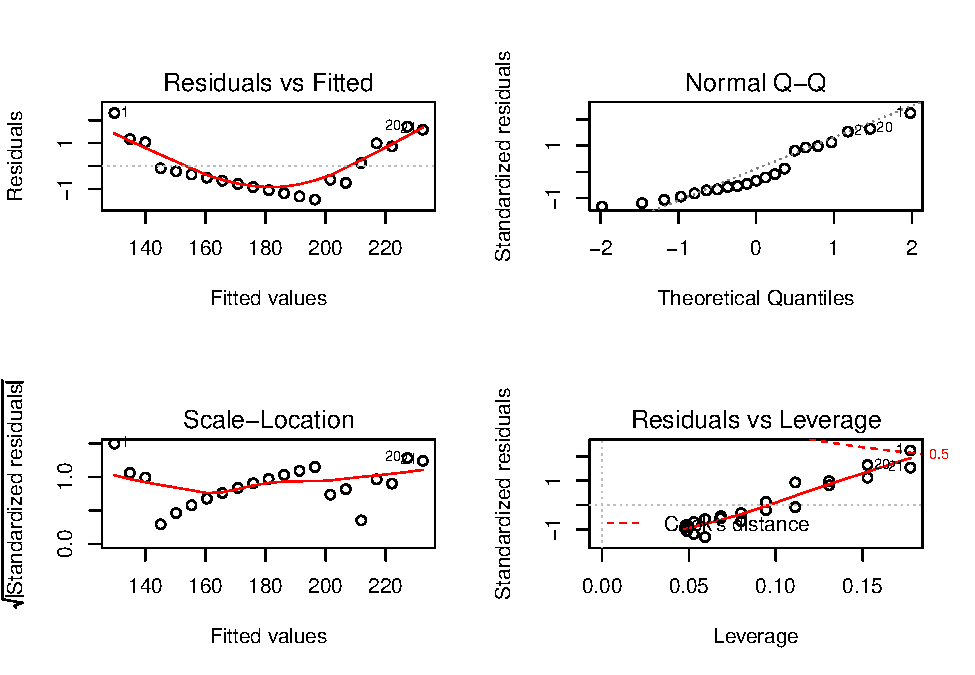
\includegraphics{Christophe_Hunt_hw5_files/figure-latex/unnamed-chunk-9-1.pdf}

From the residual plots we can tell that the residuals show constant
variance which violates the models assumptions. This model is not
actually valid for this data set.

\newpage

\section{Page 240: problem 2}\label{page-240-problem-2}

For Table 2.7, predict weight as a function of the cube of the height.

\begin{Shaded}
\begin{Highlighting}[]
\NormalTok{height3 <-}\StringTok{ }\NormalTok{height^}\DecValTok{3}
\end{Highlighting}
\end{Shaded}

Slope:

\begin{Shaded}
\begin{Highlighting}[]
\KeywordTok{slope}\NormalTok{(}\DataTypeTok{x =} \NormalTok{height3, }\DataTypeTok{y =} \NormalTok{weight)}
\end{Highlighting}
\end{Shaded}

\begin{verbatim}
## [1] 0.0003467044
\end{verbatim}

Intercept:

\begin{Shaded}
\begin{Highlighting}[]
\KeywordTok{intercept}\NormalTok{(}\DataTypeTok{x =} \NormalTok{height3, }\DataTypeTok{y =} \NormalTok{weight)}
\end{Highlighting}
\end{Shaded}

\begin{verbatim}
## [1] 59.4584
\end{verbatim}

\begin{Shaded}
\begin{Highlighting}[]
\KeywordTok{options}\NormalTok{(}\DataTypeTok{scipen=}\DecValTok{999}\NormalTok{)}
\end{Highlighting}
\end{Shaded}

The linear model y = ax + b for this data set is
\(y_{weight} = 0.000347x^3_{height}~+59.46\).

Additional measures to aid in our statistical analysis.

Error sum of squares (SSE):

\begin{Shaded}
\begin{Highlighting}[]
\KeywordTok{SSE}\NormalTok{(}\DataTypeTok{x =} \NormalTok{height3, }\DataTypeTok{y =} \NormalTok{weight)}
\end{Highlighting}
\end{Shaded}

\begin{verbatim}
## [1] 39.86196
\end{verbatim}

Total Correct Sum of Squares (SST):

\begin{Shaded}
\begin{Highlighting}[]
\KeywordTok{SST}\NormalTok{(}\DataTypeTok{y =} \NormalTok{weight)}
\end{Highlighting}
\end{Shaded}

\begin{verbatim}
## [1] 20338.95
\end{verbatim}

Regression sum of squares (SSR):

\begin{Shaded}
\begin{Highlighting}[]
\KeywordTok{SSR}\NormalTok{(}\DataTypeTok{x =} \NormalTok{height3, }\DataTypeTok{y =} \NormalTok{weight)}
\end{Highlighting}
\end{Shaded}

\begin{verbatim}
## [1] 20299.09
\end{verbatim}

Coefficient of determination \(R^2\):

\begin{Shaded}
\begin{Highlighting}[]
\KeywordTok{R2}\NormalTok{(}\DataTypeTok{x =} \NormalTok{height3, }\DataTypeTok{y =} \NormalTok{weight)}
\end{Highlighting}
\end{Shaded}

\begin{verbatim}
## [1] 0.9980401
\end{verbatim}

\newpage 

We can verify the results with the lm function in base R.

\begin{Shaded}
\begin{Highlighting}[]
\KeywordTok{library}\NormalTok{(stargazer)}
\NormalTok{lm_check <-}\StringTok{ }\KeywordTok{lm}\NormalTok{(weight ~}\StringTok{ }\NormalTok{height3)}
\KeywordTok{stargazer}\NormalTok{(lm_check, }\DataTypeTok{header =} \OtherTok{FALSE}\NormalTok{)}
\end{Highlighting}
\end{Shaded}

\begin{table}[!htbp] \centering 
  \caption{} 
  \label{} 
\begin{tabular}{@{\extracolsep{5pt}}lc} 
\\[-1.8ex]\hline 
\hline \\[-1.8ex] 
 & \multicolumn{1}{c}{\textit{Dependent variable:}} \\ 
\cline{2-2} 
\\[-1.8ex] & weight \\ 
\hline \\[-1.8ex] 
 height3 & 0.0003$^{***}$ \\ 
  & (0.00000) \\ 
  & \\ 
 Constant & 59.458$^{***}$ \\ 
  & (1.276) \\ 
  & \\ 
\hline \\[-1.8ex] 
Observations & 21 \\ 
R$^{2}$ & 0.998 \\ 
Adjusted R$^{2}$ & 0.998 \\ 
Residual Std. Error & 1.448 (df = 19) \\ 
F Statistic & 9,675.458$^{***}$ (df = 1; 19) \\ 
\hline 
\hline \\[-1.8ex] 
\textit{Note:}  & \multicolumn{1}{r}{$^{*}$p$<$0.1; $^{**}$p$<$0.05; $^{***}$p$<$0.01} \\ 
\end{tabular} 
\end{table}

\newpage

Diagnostic plots

\begin{Shaded}
\begin{Highlighting}[]
\KeywordTok{par}\NormalTok{(}\DataTypeTok{mfrow =} \KeywordTok{c}\NormalTok{(}\DecValTok{2}\NormalTok{,}\DecValTok{2}\NormalTok{))}
\KeywordTok{plot}\NormalTok{(lm_check)}
\end{Highlighting}
\end{Shaded}

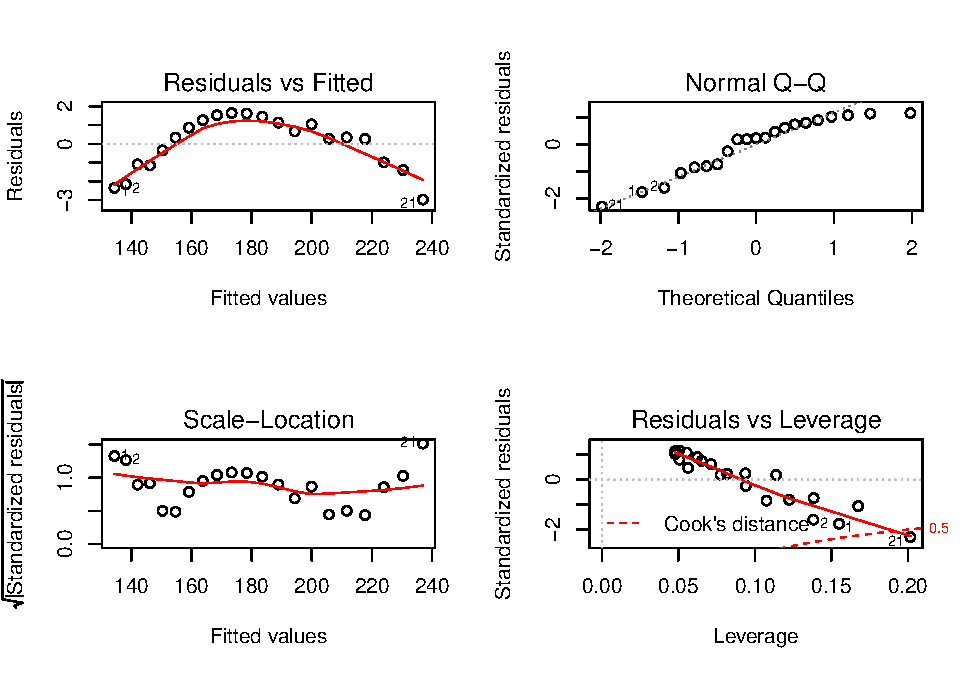
\includegraphics{Christophe_Hunt_hw5_files/figure-latex/unnamed-chunk-18-1.pdf}

There appears to be less constant variance in this residual plot, this
is the least worst model of the two using a basic linear model.


\end{document}
